\section{Concurrency control}
\subsection{Deadlocks}
Many things can block the process, lets focus on deadlocks and livelocks. We already seen what a deadlock is on the \hyperlink{lock}{\textit{diagram just above}}. We can spot deadlocks by looking at what are the necessary and sufficient conditions for deadlocks.
    \begin{tcolorbox}[gris]
        If any of these four properties are missing, deadlock will not happen:
        \begin{itemize}[left=10pt, label=\textbullet]
            \item Mutual exclusion: the system has resources protected by locks, 

                We can't be prevent this property from being true in modern systems, it's essential to prevent data corruption and data races.
            \item Hold and wait: hold a resource and wait for another,

                \begin{image}{
                        We saw this example in the \hyperlink{lock}{\textit{diagram above}}.
                    }
                    \begin{codeCenter}
                    \begin{Ccode}
objA = tbl.get(1);
objB = tb1.get(2);
synchronized(objA){
    synchronized(objB){
        ...
                    \end{Ccode}
                    \end{codeCenter}
                \end{image}
                \begin{image}{A possible solution is to say that a thread must acquire all resources before it runs. In our example it would be like going from fine-grained locking to coarse-grained locking.}
                    \begin{codeCenter}
                    \begin{Ccode}
// Lock the entire hash table
synchronized(tbl) { 
    objA = tbl.get(1);
    objB = tb1.get(2);
    ...
}
                    \end{Ccode}
                    \end{codeCenter}
                    
                \end{image}
            \item No pre-emption: there is no way for B to ``seize the lock'' from A,

                This leads to problems such as priority inversion as discussed earlier. A possible solution is to allocate priority to threads so higher priority thread can pre-empt lower priority thread and steal resources. But this approach is generally unsafe, several problems can arise like data corruption or performance overhead.
            \item Cycling waiting: A waits for B, B waits for A,

                This is the easiest and most practical to ensure this property never holds. A solution is to only allow acquiring locks in a fixed order, it means that if two objects A and B needs resources A and B, we say that both will first get (or try to get) A, and only then B. In \hyperlink{locks}{\textit{our example}}, both processors would have \lstinline!objA = tbl.get(1);!. 
        \end{itemize}
    \end{tcolorbox}
        \textbf{Challenges and applications:}

        Processes often don't know ahead of time which resources to lock, the programmer must ensure code follows ordering. Ordering locks often applied to list-like data structures, when the elements to lock are bounded, for example: multiple threads accessing a single array, sort the elements of the array in some order and allow threads to lock the elements one by one in the order. This is a very popular approach that we found inside the linux kernel.
        
    \subsubsection{Detection}
        Sometimes we can't prevent deadlocks, then, the second best approach is to detect it and kill processes involved in the deadlock. This approach require two things: an algorithm to detect deadlocks and an algorithm to recover from a deadlock.
        \begin{tcolorbox}[vert]
            A \important{resource allocation graph (RAG)} is a graph where: nodes are either resources or threads, a resource node can have multiple units and there is directed edges between threads and resource. If RAG has no directed cycle, the current state is deadlock-free. If RAG has a directed cycle: if there is only one unit per resource, there is a deadlock, for multiple units per resource, there is a possibility of deadlock.
        \end{tcolorbox}
        Let's see the notation of the one unit per resource case.
        \begin{center}
        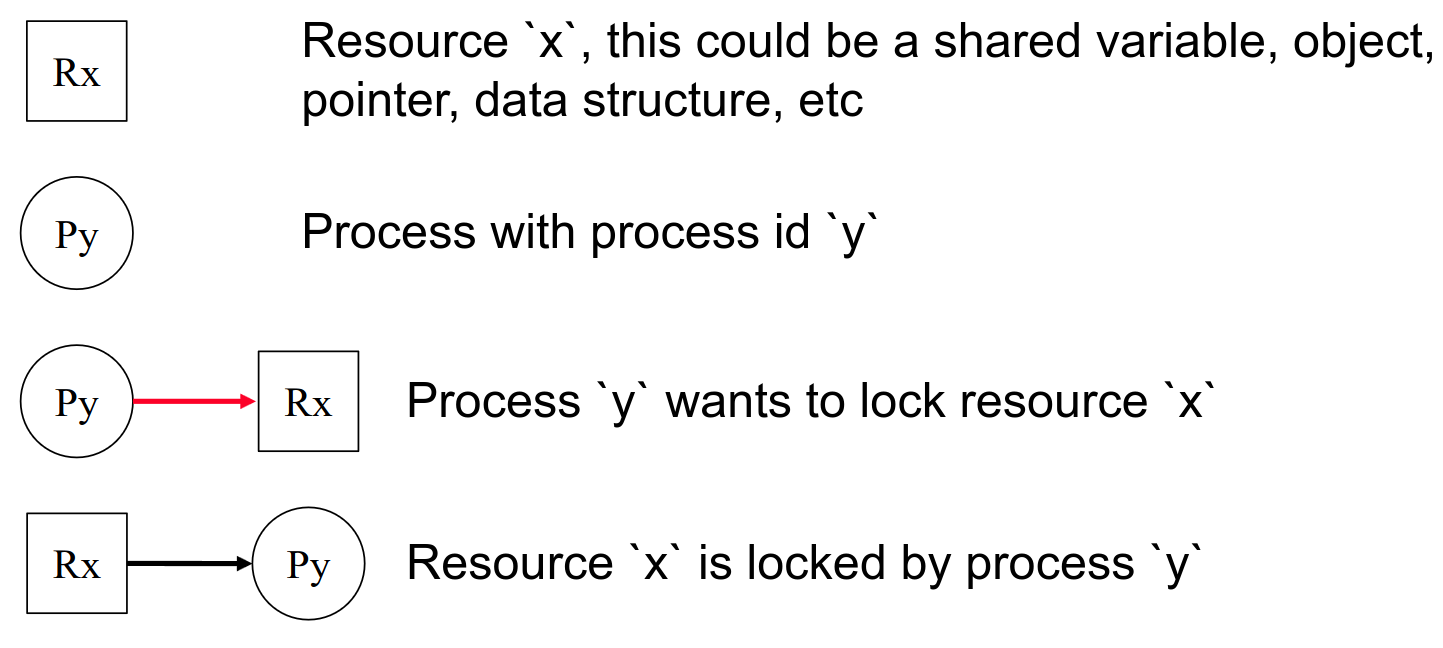
\includegraphics[width=10cm]{images/50.png}
        \end{center}
        \begin{image}{On this graph, we can see that there is a directed cycle, then the system is deadlocked!}
            \begin{center}
            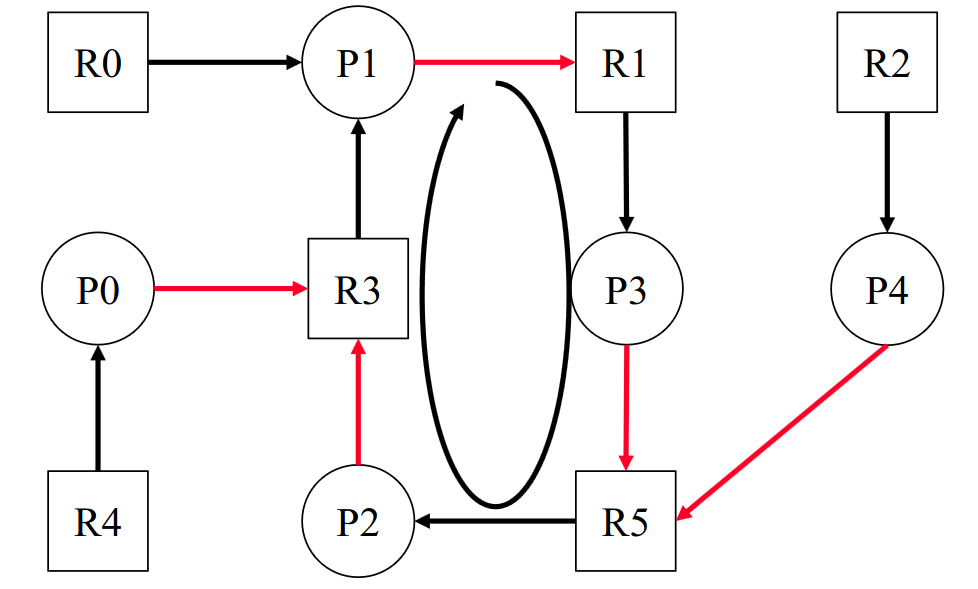
\includegraphics[width=8cm]{images/51.png}
            \end{center}
        \end{image}
        Let's see the notation of the multiple unit per resource case.
        \begin{center}
        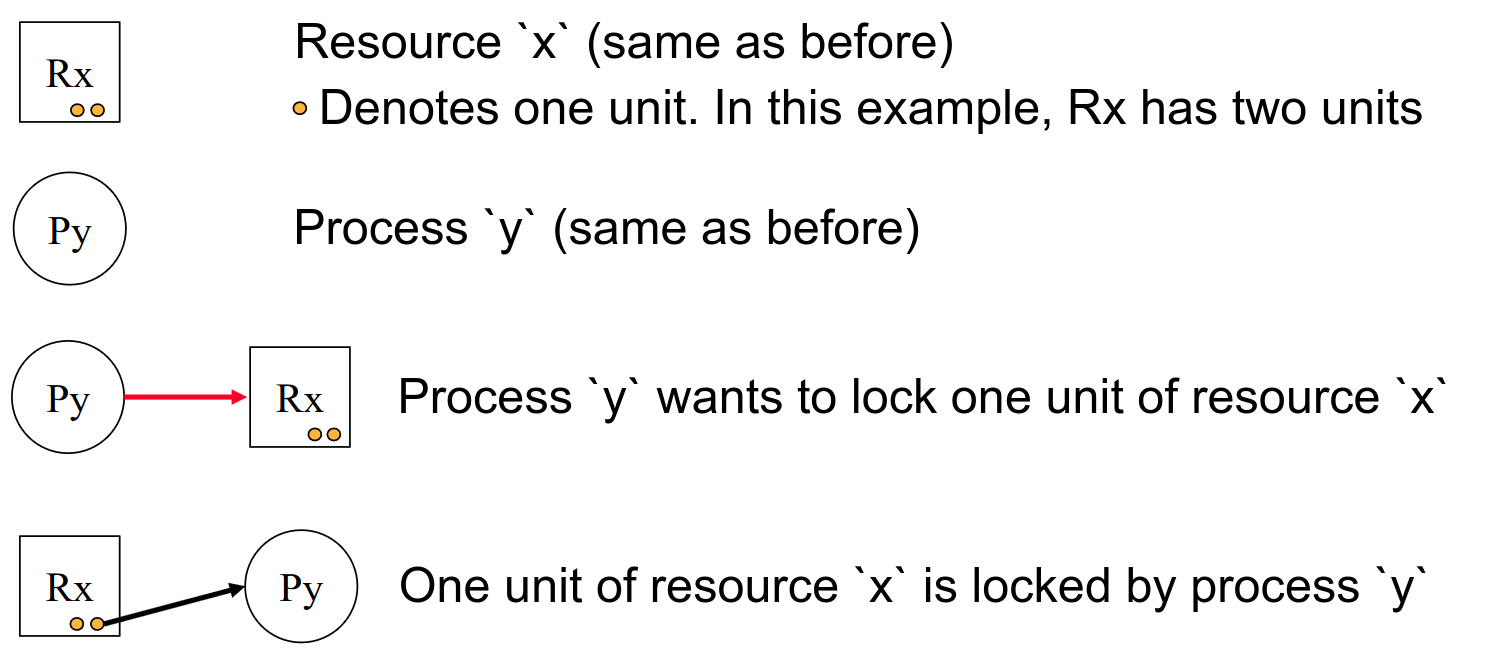
\includegraphics[width=10cm]{images/52.png}
        \end{center}
        \begin{image}{In this graph there is two directed cycle, but there may or may not be a deadlock. Let's check.}
            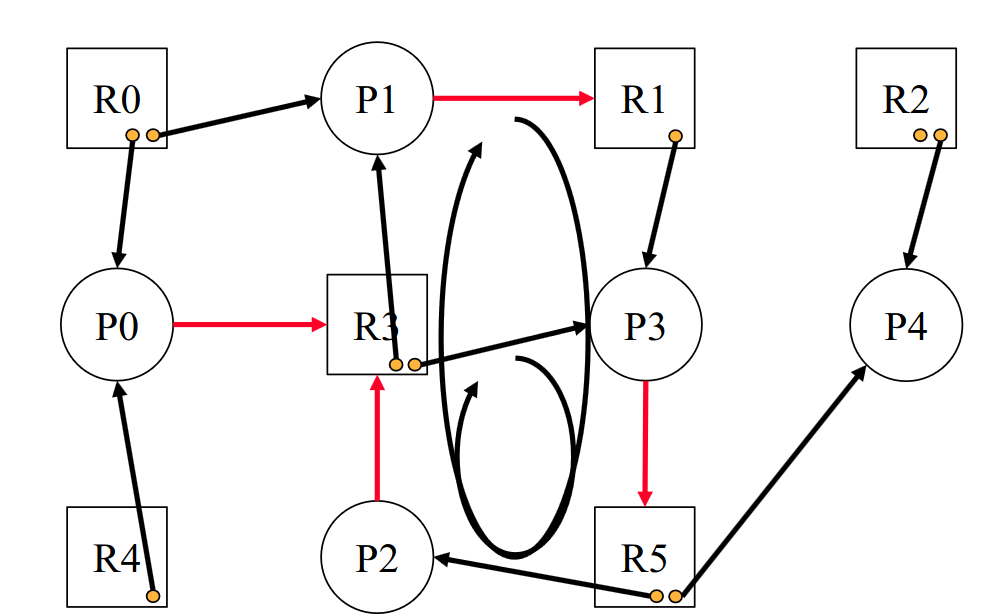
\includegraphics[width=8cm]{images/53.png
        }
        \end{image}
        Let's go step by step:
        \begin{enumerate}
            \item P4 can execute and free up resource, we can remove it from the graph, 
            \item P3 can now use R5, which has free unit, 
            \item P3 will execute next and can be removed from the graph, 
            \item P1 can now use R1 and P2 can use R3, 
            \item Both P1 and P2 can execute and be removed from the graph,
            \item Finally P0 execute.
        \end{enumerate}
        So there is no deadlocks in this system!
        \begin{tcolorbox}[violet]
            Now that we know how to detect a deadlock, what to do next? We can either terminate the process or pre-empt it.
            \begin{itemize}[left=10pt, label=\textbullet]
                \item Process termination is easy to do (simply kill all deadlocked processes) but may run into data corruption issues. 
                \item Process pre-emption is harder to do (must choose a fair victim and how much to rollback) but a more safer approach.
            \end{itemize}
        \end{tcolorbox}
        Livelocks have the same four necessary and sufficient conditions for deadlocks apply.

        
    \subsection{Transactional memory}
        Instead of writing difficult locking code, we can simply tell the runtime to make a section atomic. This is thanks to the hardware transactional memory (HTM). We only need to declare a variable so its updates will be atomic, language runtime figures it all out.
        
        \begin{tcolorbox}[vert]
            A \important{memory transaction} is an atomic and isolated sequence of memory accesses, it's supported in hardware by processor and cache hierarchy.
        \end{tcolorbox}
        
        \begin{tcolorbox}[vert]
            \important{Transactional memory (TM)} have several properties:
            \begin{itemize}[left=10pt, label=\textbullet]
                \item Atomicity: upon transaction commit, all writes take effect at once and on transaction abort, no writes take effect. 
                \item Isolation: no other processor can observe writes before commit. 
                \item Serializability: transactions seem to commit in a single serial order but the exact order is not guaranteed.
            \end{itemize}
            Contrary to locks, transactions compose gracefully.
        \end{tcolorbox}
        We need some new instructions and hardware changes to implement TM.

        \begin{tcolorbox}[gris]
            Let's introduce three Intel Haswell instructions: \lstinline!xbegin! \textrightarrow start transaction, takes pointer to fallback address in case of abort, \lstinline!xend! \textrightarrow ends transaction, \lstinline!xabort! software initiated transaction abort
        \end{tcolorbox}
        The CPU assume that no conflicts occur, it records every read and writes between \lstinline!xbegin! and \lstinline!xend! and every state is speculative (can be seen only by the core). Then the CPU checks for conflicts in the data structure (if another core is using same resources), for example, it sees a BusRdX or a BusInv matching a load (W/R) or a store (W/W) in LSQ. Check if there is another corner case (cache eviction, interruption, \ldots). Finally, on conflict, execute recovery code.
        \begin{image}{Here is an code example}
            \begin{codeCenter}
            \begin{Ccode}
xbegin recover
ld r1, mem[obj]
addi r1, #10
st mem[obj], r1
xend // commit trans.
recover:
br rec_handler
            \end{Ccode}
            \end{codeCenter}
        \end{image}
        We can observe two cases, the first one, successful:
        \begin{image}{LD OBJ and ST OBJ hit in the cache, all state remains in the pipeline and we wait until we see XEND to start committing.}
            \begin{center}
            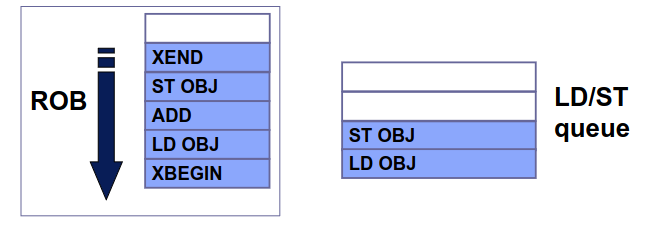
\includegraphics[width=8cm]{images/54.png}
            \end{center}
        \end{image}
        Let's see now a case with conflict:
        \begin{image}{Here we assume hat OBJ is in S state. Then the store operations induce sending a BusInv to get to M state (can be called a store miss, we can't write immediately). We then flush all instructions and execute the jump to label ``recover'' given by the user.}
            \begin{center}
            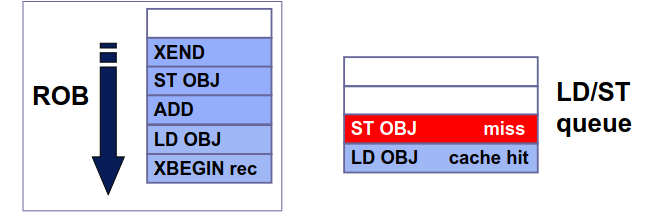
\includegraphics[width=8cm]{images/55.png}
            \end{center}
        \end{image}
        So we have to check for conflict at every operation by using coherence actions (BusRd, BusRdX, BusInv, etc\ldots).
    \subsection{Point to point synchronization}
        \begin{tcolorbox}[violet]
        Let's recall flag-based synchronization:
        
        \vspace{0.8em}
        \begin{minipage}{0.48\textwidth}
            Thread 0:
                \begin{codeCenter}
                \begin{Ccode}
// val = done = 0;
val = expensive_func();
done = 1;
                \end{Ccode}
                \end{codeCenter}
            \end{minipage}
            \begin{minipage}{0.48\textwidth}
            Thread 1:
                \begin{codeCenter}
                \begin{Ccode}
// done = 0;
while(!done){ }
... = val;
                \end{Ccode}
                \end{codeCenter}
            \end{minipage}
        \end{tcolorbox}
        It assumes sequential consistency!
        \begin{tcolorbox}[vert]
           \important{Barriers} introduce planned stalls in threads, like wait for all threads to read input before start. They use flags.
        \end{tcolorbox}
        Here is the idea behind the implementation of the barrier:
        \begin{image}{
                \begin{enumerate}[left=10pt]
                    \item Clear the flag, tell all incoming threads to wait,
                    \item Every arriving thread increments \lstinline!counter!, 
                    \item Last thread sees \lstinline!counter == num\_threads!,
                    \item Set the flag, all threads leave,
                \end{enumerate}
            }
            \begin{codeCenter}
            \begin{Ccode}
struct Barrier_t {
    Lock aLock;
    int counter;
    int flag;
};
            \end{Ccode}
            \end{codeCenter}
        \end{image}
        \begin{tcolorbox}[rouge]
        A basic implementation of this algorithm wouldn't work because some thread can arrive to a new barrier while others haven't left the one before, so there would be a deadlock. That's why we need to keep a private copy of the flag, the first thread to arrive writes its private copy (\lstinline!int local_sense = 0; //private!). It looks like this:
        \begin{codeCenter}
        \begin{Ccode}
void senseBarrier(Barrier_t* b, int num_threads) {
    local_sense = !(local_sense); // (Step 1)
    lock(b->aLock);
    int num_waiting = ++(b->counter); // (Step 2)
    if( num_waiting == num_threads ) { // (Step 3)
        unlock(b->aLock);
        b->counter = 0;
        b->flag = local_sense; // (Step 4)
    } else {
        unlock(b->aLock);
        while( b->flag != local_sense ); // spin
    }
} 
        \end{Ccode}
        \end{codeCenter}
        \textbf{Traffic on bus:} $O\left(P\right)$, \space \space \textbf{Latency: }$O\left(P\right)$.
        \end{tcolorbox}
        \begin{tcolorbox}[vert]
            But we can achieve a $\log\left(P\right)$ latency with \important{combining trees}! The strategy is to acquire when the processor arrives at barrier, performs \lstinline!atomicIncr(parent.counter)!, and the process recurses to the root. The idea is that when every children of a parent are arrived, the parent (who is also a children) can increment its own parent, until we reach the root. 
        \end{tcolorbox}
        \begin{center}
            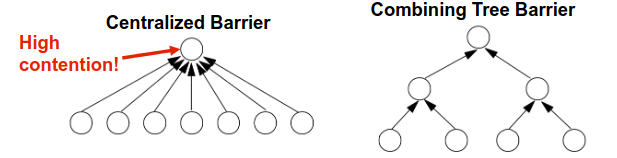
\includegraphics[width=10cm]{images/56.png}
        \end{center}
        \begin{tcolorbox}[gris]
            
        
        \textbf{Examples of locks in OpenMP:}
        \begin{itemize}[left=10pt, label=\textbullet]
            \item \lstinline!omp_init_lock(omp_lock_t *)! : initializes the lock variable passed, lock is not held by the initializing thread, 
            \item \lstinline!omp_destroy_lock(omp_lock_t *)! : disassociates the given lock variable from any locks, 
            \tem \lstinline!omp_set_lock(omp_lock_t *)! : waits until the lock is available, then acquires the lock, 
            \item \lstinline!omp_unset_lock(omp_lock_t *)! : releases the lock, 
            \item \lstinline!omp_test_lock(omp_lock_t *)! : attempts to set a lock, but does not block if the lock is unavailable.
        \end{itemize} 
        
        \begin{codeCenter}
        \begin{Ccode}
omp_lock_t lock;
omp_init_lock(&lock);

#pragma omp parallel num_threads(4)
{
    int tid = omp_get_thread_num( );
    int i;
    for (i = 0; i < 3; ++i){
        omp_set_lock(&lock);
        printf("T %d: begin locked region\n", tid);
        printf ("T %d: end locked region\n", tid);
        omp_unset_lock(&lock);
    }
}

omp_destroy_lock(&lock);
        \end{Ccode}
        \end{codeCenter}
        \end{tcolorbox}
